% This is LLNCS.DEM the demonstration file of
% the LaTeX macro package from Springer-Verlag
% for Lecture Notes in Computer Science,
% version 2.2 for LaTeX2e
%
\documentclass[oribibl]{llncs_Ibergrid2013}
%
\usepackage{makeidx}  % allows for indexgeneration
%
%\usepackage[dvips]{graphicx}
%
\usepackage{epsfig}
%\usepackage{cite}
\usepackage{url}
\usepackage{microtype}
\usepackage[english]{babel}
\usepackage{graphicx}
\usepackage{eurosym}
\usepackage{url}
\usepackage{multirow}
\usepackage{listings}
%\usepackage{natbib}

%%%% TABLES
\usepackage{dcolumn}
\newcolumntype{d}{D{.}{.}{-1}}
%%
\usepackage{booktabs}
%%
\usepackage{longtable}
\setlength{\doublerulesep}{0pt}
%%
\usepackage{multirow}
\newcommand{\mr}[1]{\multirow{2}{2em}{#1}}
%%
%\usepackage{array}


\begin{document}
%
\frontmatter          % for the preliminaries
%
\pagestyle{headings}  % switches on printing of running heads
\addtocmark{Running Big Data on the EGI Federated Cloud} % additional mark in the TOC
%
\mainmatter              % start of the contributions
%
\title{Running Big Data on the EGI Federated Cloud}
%
\titlerunning{Big Data on FedCloud}  % abbreviated title (for running head)
%                                     also used for the TOC unless
%                                     \toctitle is used
%
\author{J.~L\'opez Cacheiro\inst{1}, A.~Sim\'on\inst{1}, J.~Villasuso\inst{1}, E.~Freire\inst{1}, R.~Rosende\inst{1}, I.~D\'iaz\inst{1}, A.~Feij\'oo\inst{1}, P.~Rey\inst{1}, C.~Fern\'andez\inst{1} and B.~Parak\inst{2}}
%
%\authorrunning{First Author et al.}   % abbreviated author list (for running head)
%
%%%% modified list of authors for the TOC (add the affiliations)
\tocauthor{First Author (Institution of first author's affiliation),
Second Author (Institution of second author's affiliation)}
%
\institute{Fundaci\'on Centro de Supercomputaci\'on de Galicia, Spain\\
	\email{grid-admin@cesga.es}
	\and
	CESNET, Czech Republic\\
	\email{boris.parak@cesnet.cz}
}




\maketitle              % typeset the title of the contribution

\begin{abstract}
Big Data is an emerging technology that could benefit from existing developments in cloud technologies. In this paper we evaluate the suitability of FedCloud--the federated cloud infrastructure developed inside EGI--to perform Big Data analytics using Hadoop. Due to the size of the tests performed, they represent also a real benchmark of the performance of FedCloud under heavy usage conditions, providing the first results about the scalability of the system.

% usability
% estability

\end{abstract}

%
\section{Introduction}
\label{sect-introduction}
% Big Data 
% Hadoop 
% Cloud 
% Federated cloud
% FedCloud

% Big Data on federated Cloud
% Amazon Hadoop service
% BC-PDM: Because of the limitations of the current system, China Mobile initiated an experimental project to develop a parallel data mining tool set on Hadoop and evaluated it against its current system. They named the project Big Cloud–based Parallel Data Mining (BC-PDM) [Hadoop in Action Book page 269]

% Short summary and main objective of the work
Nowadays, the possibility to run Big Data calculations over federated clouds is a topic that is attracting the interest of the research community. Federation of resources poses serious challenges both from the cloud and Big Data perspectives. The aim of this paper is to evaluate the suitability of the FedCloud federated cloud infrastructure that it is being developed inside EGI to run typical Big Data analytics using Hadoop. 

% Big Data
Big Data is one of the buzzwords that sounds everywhere, the Big Data community is working to extend the scalability of traditional databases (RDMS) using new technologies based on a share-nothing architecture. In this arena, one of the most well-known solutions is Hadoop~\cite{hadoop}, an open-source framework that implements the MapReduce computational paradigm on top of a parallel HDFS filesystem.

% Previous attempts to run Hadoop on the Cloud

% Amazon EC2

% FedCloud
The EGI Federated Cloud Task Force~\cite{fedcloud} started its activity in September 2011 with the aim of creating a federated cloud testbed--named FedCloud--to evaluate the utilization of virtualized resources inside the EGI production infrastructure. Even if the development is still in progress, the testbed is already available for experimentation by the different user communities. A more detailed description of the EGI FedCloud infrastructure is given in~\cite{egifedcloud}.


% Aim & structure 
The aim of our work is to do an initial assessment of the suitability of FedCloud to run Hadoop through a series of real-world benchmarks. The paper is organized as follows: in Section~\ref{sect-methodology} we describe the methodology used to deploy Hadoop inside the FedCloud federated cloud infrastructure; in Section~\ref{sect-results} we show the results obtained after running several deployment and execution benchmarks based on the analysis of two common data sources: Encyclop{\ae}dia Britannica and Wikipedia; finally in Section~\ref{sect-conclusions} we present the main conclusions of this work, summarizing the main problems encountered as well as outlining the future steps that could be taken to provide Hadoop as a on-demand service in FedCloud.


\section{Methodology}
\label{sect-methodology}
In this Section we describe the methodology that we have followed to deploy a Hadoop cluster instance inside the FedCloud federated cloud infrastructure. Basically, three steps were involved in the process: 
\begin{enumerate}
\item \emph{Cluster startup}: obtaining the resources necessary to form the cluster from each of the sites in FedCloud
\item \emph{Hadoop configuration}: configuring the Hadoop cluster
\item \emph{Benchmark execution}: loading the data sets and running various MapReduce jobs
\end{enumerate}
Each of these steps is described in more detail in the following subsections.

\subsection{Cluster startup}
\label{ssect-cluster}

A general overview of the overall cluster startup process is given in Figure~\cite{fig:client}.
% VM template & Marketplace
In order to simplify the later configuration, we created a customized virtual machine (VM) image template that includes all the software necessary to run Hadoop. This image is based on Scientific Linux 6.4 and contains the following customizations:
\begin{itemize}
\item \emph{Firewall:} iptables is configured to allow inter-cluster communication.
\item \emph{SSH:} enable root access through ssh public key authentication (\emph{authorized\_keys}).
\item \emph{Modules:} we make use of the Modules package to simplify the deployment of the software needed to run Hadoop.
\item \emph{Java:} we use Oracle Java JDK 1.6.0\_33 because it offers better performance than the OpenJDK version. It is also configured through Modules to allow simple migration to other Java versions.
\item \emph{Hadoop:} both Hadoop-1.0.3 and Hadoop-1.0.4 are included. The configuration using Modules makes easy to include additional versions and decide the one we want to use when starting the Hadoop cluster.
\end{itemize}


This customized image was registered in the EGI Marketplace~\cite{marketplace} which provides a common place where where we can can store images. Unfortunately, the Marketplace does not store the VM images into a common repository, it just shows which resource providers (RPs) have the VM image available at their endpoint. This means that each RP has to manually download the image to his local site in order to make it available at his endpoint. Currently there is no automated way to perform this step so the distribution of the VM template to all the sites is a time consuming effort that involves contacting the FedCloud administrators of each each site. It should be noted that a vanilla SL6 or Debian image from the Marketplace could have also used instead of using our customized image, which main purpose was just to allow us to pre-install software.


% Client: rOCCI + VOMS
The next step is to instantiate the virtual machines that will form the Hadoop cluster, for this purpose we make use of the new implementation of the OCCI 1.1 specification under rOCCI~\cite{rocci} as well as our VOMS proxy credentials. The new rOCCI implementation provides several advantages like the fact that we are able to avoid the previous issue that all user certificates request are mapped to a single ONE\_USER account.
Additionally, the usage of VOMS over plain X509 auth greatly simplifies the access to the different sites that form FedCloud without the need to request each site to give access to our X509 certificate's DN.

Unfortunately FedCloud does not count with a workload management system, so each VM creation request must be sent to the appropriate endpoint. This means that we have to take care ourselves of the partitioning of the cluster between the different FedCloud sites.

%\begin{figure}[h]
%\centering
%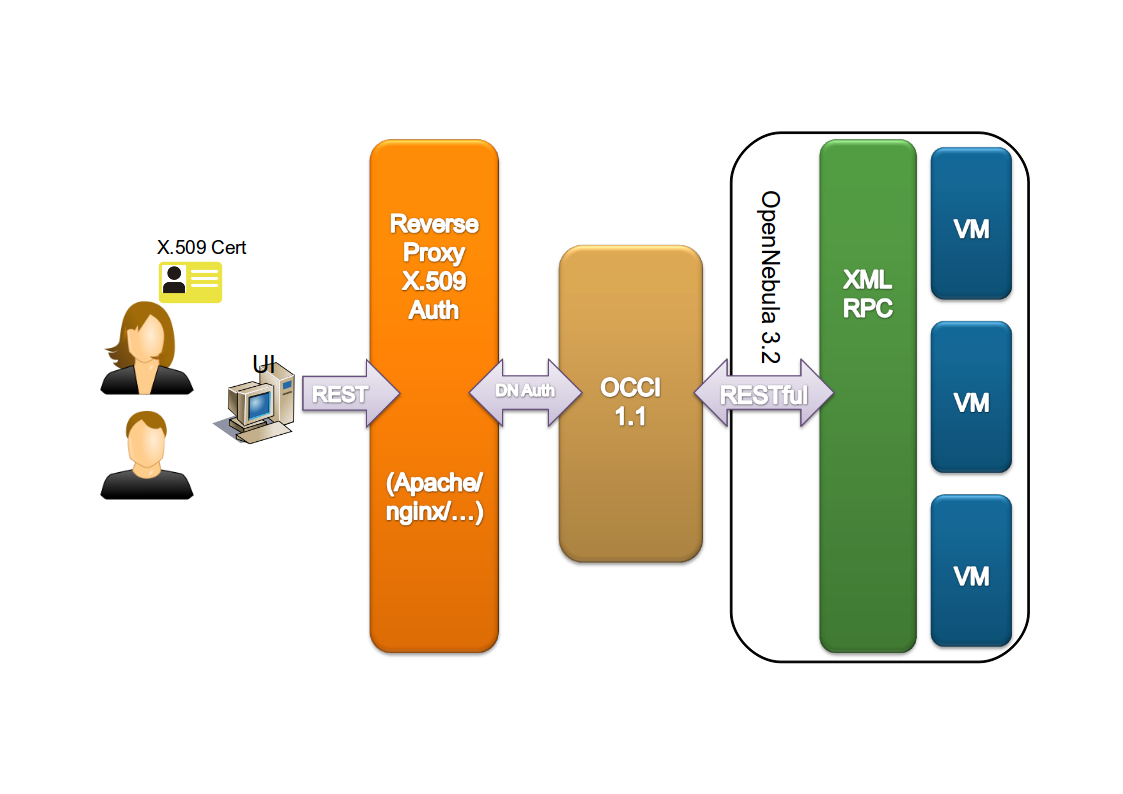
\includegraphics[width=0.8\textwidth]{figures/occi_opennebula.png}
%\caption{OCCI 1.1 server and x509 auth for OpenNebula.}
%\label{fig:occi1}
%\end{figure}

\begin{figure}[h]
\centering
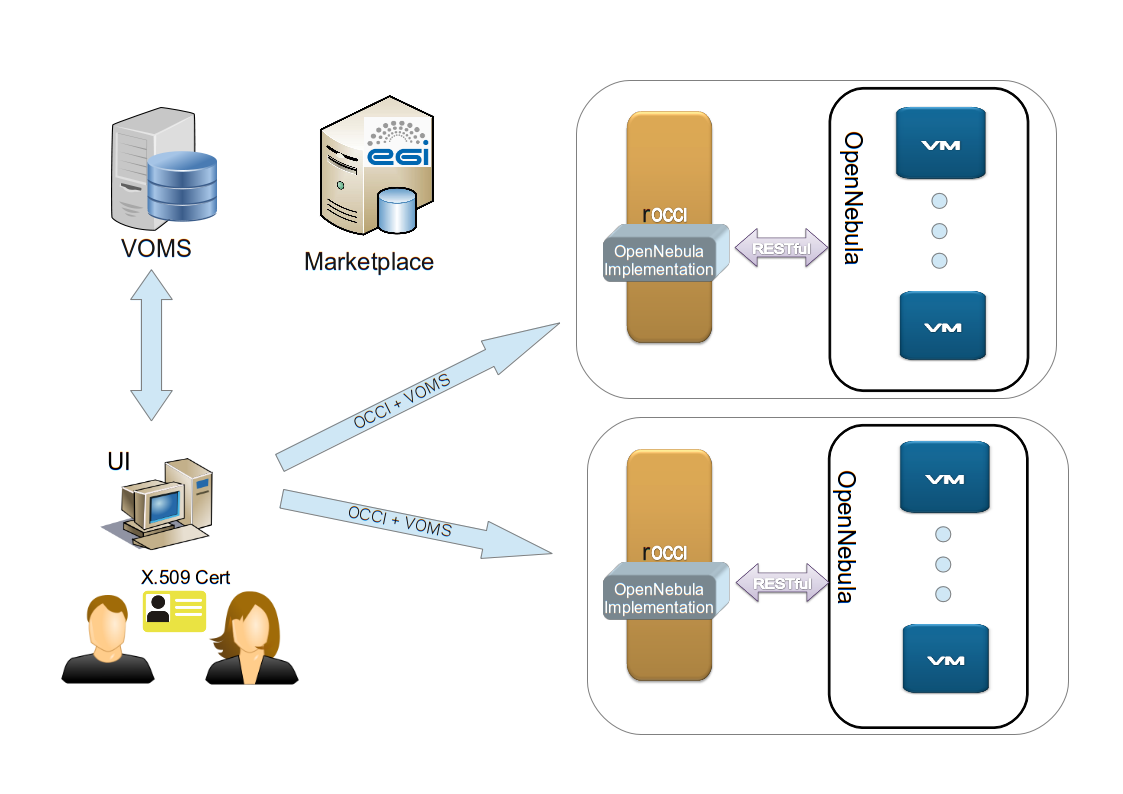
\includegraphics[width=\textwidth]{figures/client-v2.png}
\caption{Cluster startup process using rOCCI and VOMS from a single UI.}
\label{fig:client}
\end{figure}

% Resources used
About the resources used by each of the instances, in order to increase the concurrent number of VMs, we used small size VM instances with 1GB of RAM and 1 CPU.


\subsection{Hadoop configuration}
\label{ssect-hadoop}
% Basics about Hadoop services needed: hadoop-master, slaves
After having the cluster running, the next step is to prepare the nodes to run Hadoop. As it has been explained in \ref{ssect-cluster}, the software necessary is already pre-deployed in the nodes so we only have to configure Hadoop. 

Our Hadoop cluster will consist of one \emph{master} node and a variable number of \emph{slave} nodes depending on the size of the cluster. For example in the case of a 101 node cluster, one node will be configured as master and the remaining 100 as slaves. The master node will run the \emph{namenode}, \emph{secondarynamenode} and \emph{jobtracker} services and each of the slaves will run just one \emph{tasktracker} and one \emph{datanode} services
due to the fact that we are using small VM instances with just 1GB of RAM and 1 CPU we decide to run just one tasktracker and one datanode per slave. 

 The tuned configuration parameters are given in Table \ref{table:conf}. The column type identifies the configuration file where the parameter is set, the complete configuration files can be found at~\cite{scripts}.
% TODO: figure showing the master/slave setup and the services
% Hadoop configuration
%% Hadoop 1.0.3
%% Oracle Java JDK 1.6.0_33
%% Modules

These parameters have been configured to adapt the Hadoop cluster to resources available--1GB of RAM and 1 CPU per node--. The $dfs.replication$ parameter indicates how many copies we want to store of each block, in this case we use three replicas that will allow different nodes to execute the same mapreduce tasks--speculative execution--mitigating the performance degradation that could be experienced in a heterogeneous cluster with VMs running under hypervisors with different load conditions. The $mapred.tasktracker.map.tasks.maximum$ and $reduce.tasks.maximum$ are set to 1 because we only have 1 CPU available to run both services and the HADOOP\_HEAPSIZE is set to 512MB to allow both running at the same time without exhausting the node's memory. The number of reduce tasks, $mapred.reduce.tasks$, is set to 95\% of the number of slaves in the Hadoop cluster. 

As we will see in Section \ref{ssect-execution} our Hadoop installation will cope with two very different use cases that influence our decission about the $dfs.block.size$ values to use. In the case of the Encyclop{\ae}dia Britannica's use case the block size is set to 1MB and in the Wikipedia's use case, that uses a much larger data set, to 64MB. Under this conditions both use cases generate less than 700 total mapreduce tasks which can be handled well by our hadoop master node which has only 1GB of RAM and 1 CPU.


%% table with the parameters used
% TODO: complete the table
\begin{table}[h!]
\caption{Tuned Hadoop configuration for small VM instances. It includes both the HDFS and MapReduce parameters used.}
\label{table:conf}
%
\vspace{-0.5em}
%
\begin{center}
\begin{tabular}{ccc}
\toprule
%Parameter				& Type\tablenotemark[a] & Value	 	\\
Parameter				& Type 			& Value	 	\\
\midrule
$fs.inmemory.size.mb$			& core-site		& 200MB	 	\\
$io.file.buffer.size$                  	& core-site		& 128KB  	\\
$mapreduce.task.io.sort.factor$ 	& core-site		& 100	 	\\
$mapreduce.task.io.sort.mb$ 	 	& core-site		& 100	 	\\
$mapred.tasktracker.map.tasks.maximum$ 	& mapred-site		& 1	 	\\
$mapred.tasktracker.reduce.tasks.maximum$ & mapred-site		& 1	 	\\
$mapred.reduce.tasks$ 			& mapred-site		& $0.95\times$\emph{num.~slaves} \\
$dfs.datanode.du.reserved$ 		& hdfs-site		& 1GB	 	\\
$dfs.block.size$ 			& hdfs-site		& 1MB / 64MB 	\\
$dfs.replication$ 			& hdfs-site		& 3	 	\\
HADOOP\_HEAPSIZE            	 	& hadoop-env   		& 512MB 	\\
%HADOOP\_OPTS                	 	& hadoop-env   		& $-XX:+UseParallelGC$ 	\\
%                             	 	&              		& $-Djava.net.preferIPv4Stack=true$ 	\\
%
%(1,5,0)		& 0.0645	& 0.0689\tablenotemark[d]	& $2 \times 10^{-4}$		\\
%
\bottomrule
\multicolumn{3}{c}{\rule{0.98\textwidth}{0em}}\\
%\rule{0.3\textwidth}{0cm} & \rule{0.2\textwidth}{0cm} &  \\
\end{tabular}
\end{center}
%\vspace{-3.5em}
%\tablenotetext[a] {Identifies the configuration file where the parameter is set, the complete configuration files can be found at \url{https://github.com/grid-admin/hadoop}}
\end{table}


%% TODO: Explain the values of the parameters used


\subsection{Benchmark execution}
\label{ssect-execution}

In order to evaluate the suitability of FedCloud to perform Big Data analytics using Hadoop we selected two use cases which are quite representative of a broad range of jobs that could be performed in a Hadoop cluster. The benchmarks were run both in a federated cluster deployment and in a one-site-only cluster deployment, allowing us to compare the results and analyse the expected degradation when using remotely distributed resources.

% Encyclopaedia Britannica 1911: 176MB
%% -put (5 runs)
%%% Upload from hadoop-master
%% wordcount (5 runs)

% Wikipedia: 41GB
%% -put (1 run)
%%% Upload from UI (hadoop-master does not have enough space to store it)
%% wordcount (5 runs)


The first use case is based in the Encyclop{\ae}dia Britannica\cite{britannica} data set--the 1911 version that is already in the public domain--. This represents a rather small data set of just 176MB, so that this use case can be considered as a small scale benchmark that will serve to evaluate the expected degradation in performance due to fact that we will be using federated resources located at different sites. The data set is downloaded directly from the master node and later on it is distributed from there to the slaves, what is called a \emph{put} operation in Hadoop argon. This use case has a great overload due to the creation of rather small mapreduce tasks that will stress the communication system because it uses a rather small block size of just 1MB, so each map operation has little to process.

The second use case is based in the Wikipedia\cite{wikipedia} data set. This represents a much larger data set comprising 41GB, so it can be considered a more realistic benchmark of a Big Data application. Due to the size of the data set the files could not be downloaded directly in the master node so the \emph{put} operation is done directly from our local Hadoop client located at CESGA. This use case will incur in a lower task creation penalization because it uses a larger block size of 64MB, so each map task will take much longer than the time needed for its creation.


The benchmarks are run for different cluster sizes that range from 10 to 101. In all the benchmarks we measure two parameters:
\begin{enumerate}
\item \emph{The put time:} the time to load the files into the Hadoop HDFS filesystem 
\item \emph{The wordcount time:} the time to perform a simple wordcount mapreduce job that computes the number of occurrences of each word over the complete data set. 
\end{enumerate}
All the measurements where repeated at least 5 times in order to evaluate the variability of the results, the only exception were the \emph{put} times for the Wikipedia that due to its duration could only be run once.

\section{Results}
\label{sect-results}

Following the methodology described in the previous Section we deployed Hadoop inside FedCloud and executed the benchmarks mentioned in subsection \ref{ssect-execution}. In this Section we present the benchmark results obtained for the two selected use cases: Encyclop{\ae}dia Britannica and Wikipedia.

The first results to consider are those related to the cluster startup process described in Section \ref{ssect-cluster}. In this case we are dealing with the instantiation of a number of VMs that ranges from 10 to 101 so it can also serve as a stress test of the FedCloud rOCCI framework as well as the underlying cloud management platform--currently only OpenNebula is supported by rOCCI.


After some initial VM deployment tests we discovered that most of the sites involved in FedCloud were misconfigured or did not support rOCCI, and only two sites were providing a working rOCCI endpoint: CESGA and CESNET. So we deployed our federated infrastructure using these two sites.

The startup times for each cluster deployment varied and the most representative ones are those obtained for the larger deployment, the 101 node cluster. In this case, the time needed by the rOCCI client to return all the resource endpoints corresponding to each VM ranged from 71 to 86 minutes. This is just the time to get the identifier corresponding to each VM instance, actually to have all the VMs running took even longer, around 80 minutes more. So the total cluster startup time ranged from 2.5 to 3 hours. But this was not the main issue encountered, the main problem was that some of the rOCCI requests failed with an \emph{execution expired} error and some of the VMs did not start--in the worst case 21 out of 101 failed.
%\begin{verbatim}
%An error occurred! Message: execution expired
%An error occurred! Message: HTTP Response status: [500] Internal Server Error!
%\end{verbatim}
We started to see this type of errors as soon as we tried to deploy, in a sequential way, more than 20 VMs at CESGA. In CESNET we could not do this analysis because there were only 10 VM slots available due to a restriction in the amount of public IPs that they had available.

Trying to understand the source of this issue we tracked the performance of the OpenNebula frontend during the cluster startup. As it can be seen in Figure \ref{fig:on} the frontend experiences a high load several minutes after the start of the cluster deployment, this causes it to respond slower, probably producing the rOCCI execution expiration errors mentioned above. Looking at the processes in the OpenNebula frontend, we could see that this increase in the load is mainly due to the scp processes launched to copy the image template to the OpenNebula nodes, more than 20 simultaneous scp processes seem to affect considerably the system performance, reducing its response times considerably.

% * Deploying 101 VMs:
%{{{
%[jlopez@test13 ~]$ time ./deploy_cluster_voms.sh &> deploy_cluster_voms.log
%
%real	71m31.677s
%user	1m43.104s
%sys	0m25.706s
%
%[jlopez@test13 ~]$ wc -l machines/pending
%98 machines/pending
%
%}}}
%

% Screenshot ganglia: 100 VMs deployment
\begin{figure}[t!]
\centering
%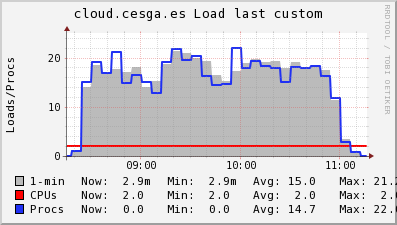
\includegraphics[width=0.74\textwidth]{figures/ON_load-complete.png}
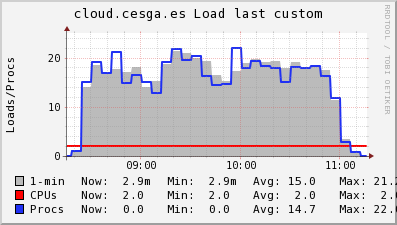
\includegraphics[width=0.6\textwidth]{figures/ON_load-complete.png}
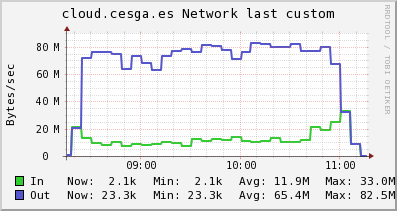
\includegraphics[width=0.6\textwidth]{figures/ON_network-complete.png}
\caption{OpenNebula frontend load and network usage graphs taken from Ganglia during the deployment of the 101 nodes cluster.}
\label{fig:on}
\end{figure}


Another problem we encountered was that FedCloud does not count with a workload management system, so each VM creation request must be sent to the appropriate endpoint. This means that we have to take care in advance of the partitioning of the cluster between the different FedCloud sites. In our case we choose to run 10 VM at CESNET--the maximum possible at the time of the benchmarks--and the rest of them at CESGA--ranging from 10 to 91.

Once the cluster is deployed we proceed to configure Hadoop. In this case the only problem encountered was due to the global firewall rules at each site that blocked Hadoop communications. Once this issue was addressed the Hadoop cluster started flawlessly. The time involved to configure and start the Hadoop cluster was really short, taking less than 1 minute in the larger setup with 101 nodes, so it is almost irrelevant in the total cluster startup time when considering the almost 3 hours needed for VM instantiation.

%Finally we proceeded with the execution of the specific Big Data use cases described in Section \ref{ssect-execution}.

% Results Enc. Britannica
In Table \ref{table:britannica} we show the results obtained for the Encyclop{\ae}dia Britannica use case. All measurements are repeated 5 times and the average and standard deviation are displayed, allowing to have an estimation of the variability involved in the measurement. As it can be seen even if the block size used in this case is very small (1MB), the wordcount map reduce job scales really well and the overhead introduced by the federated cluster is small, being in general in order of 10-15\%, and 28\% in the worst case that corresponds to the 101 cluster. This is mainly due to the large overhead that mapreduce task creation and distribution imposes in this use case, especially in the larger cluster sizes that involve more reduce tasks--we are using a number of reduce tasks equal to the 95\% of the total number of slaves.

As expected the put times are much lower in one-site-only scenario because in this case the connection between all the VMs is much faster because all of them are generally located in the same data centre.

%% Table results Enc. Britannica
\begin{table}[h!]
\caption{Benchmark times obtained for the Encyclop{\ae}dia Britannica use case. Both the average time and standard deviation are reported. Federated times where measured in a federated cluster that included resources both from CESGA and CESNET; all one-site-only times where obtained in a one site deployment at CESGA except the 10 node cluster indicated in the second row that run at CESNET. }
\label{table:britannica}
%
\vspace{-0.5em}
%
\begin{center}
\begin{tabular}{ccccc}
\toprule
%Parameter				& Type\tablenotemark[a] & Value	 	\\
%Cluster size				& put (s) Local		& put (s)		& wordcount (s) 	& wordcount (s) 	\\
					& \multicolumn{2}{c}{Federated} 		& \multicolumn{2}{c}{One-site-only} \\
Cluster size				& put (s)		& wordcount (s) 	& put (s)		& wordcount (s)\\
\midrule
10 (CESGA)             			&        		&               	& $47\pm2$		& $169\pm1$\\
10 (CESNET)          			& 			&  			& $9.5\pm0.2$		& $160\pm1$\\
21                   			& $235\pm12$		& $108\pm2$     	& $37\pm1$		& $97\pm1$\\
31                   			& $189\pm4$		& $90\pm2$      	& $36\pm2$		& $78\pm2$\\
41                   			& $190\pm11$		& $81\pm4$      	& $33\pm2$		& $71\pm3$\\
51                   			& $133\pm7$		& $73\pm3$      	& $33\pm1$		& $66\pm2$\\
101                  			& $94\pm7$		& $67\pm22$      	& $33\pm4$		& $52\pm5$\\
%
\bottomrule
\multicolumn{5}{c}{\rule{0.98\textwidth}{0em}}\\
\rule{0.2\textwidth}{0cm} & \rule{0.2\textwidth}{0cm} & \rule{0.2\textwidth}{0cm} &  \rule{0.2\textwidth}{0cm} & \\
\end{tabular}
\end{center}
%\vspace{-3.5em}
%\tablenotetext[a] {Identifies the configuration file where the parameter is set, the complete configuration files can be found at \url{https://github.com/grid-admin/hadoop}}
\end{table}



% Results Wikipedia
In Table \ref{table:wikipedia} we show the results obtained for the Wikipedia use case. It should be noted that due to the high duration of the transfers, we did not repeat the put measurements 5 times, and only the wordcount measurements were repeated. Also due to the longer duration of the benchmarks we only used the two larger cluster sizes: 51 and 101.

In this case the wordcount mapreduce results are quite surprising because the federated cluster instance is able to outperform the one-site-only instance in both scenarios. This is attributed mainly to the faster execution of the benchmark in CESNET nodes compared to CESGA nodes--CESNET VMs use Xen paravirtualization and a faster CPU whereas CESGA VMs use KVM and QEMU--. In this case the relative overhead due to mapreduce task creation is much lower than in the previous use case because we are using a much larger block size of 64MB.

The put times are much larger in the federated cluster due to the fact that the amount of data to transfer is much larger--HDFS stores three copies of the Wikipedia, 42GB each, so that the available bandwidth between the VMs and the UI located at CESGA plays a key role, being much lower in the case of CESNET VMs.

%% Table results Wikipedia
\begin{table}[h!]
\caption{Benchmark times obtained for the Wikipedia use case. Both the average time and standard deviation are reported except for the put times that where only measured once for each deployment. Federated times where measured in a federated cluster that included resources both from CESGA and CESNET; all one-site-only times where obtained in a one site deployment at CESGA. }
\label{table:wikipedia}
%
\vspace{-0.5em}
%
\begin{center}
\begin{tabular}{ccccc}
\toprule
%Parameter				& Type\tablenotemark[a] & Value	 	\\
%Cluster size				& put (s) Local		& put (s)		& wordcount (s) 	& wordcount (s) 	\\
    					& \multicolumn{2}{c}{Federated} 		& \multicolumn{2}{c}{One-site-only} \\
Cluster size				& put (s)		& wordcount (s) 	& put (s)		& wordcount (s)\\
\midrule
51                   			& $19190$		& $1001\pm39$      	& $6705$		& $1347\pm117$\\
101                  			& $13208$		& $705\pm14$      	& $5665$		& $725\pm18$\\
%
\bottomrule
\multicolumn{5}{c}{\rule{0.98\textwidth}{0em}}\\
\rule{0.2\textwidth}{0cm} & \rule{0.2\textwidth}{0cm} & \rule{0.2\textwidth}{0cm} &  \rule{0.2\textwidth}{0cm} & \\
\end{tabular}
\end{center}
%\vspace{-3.5em}
%\tablenotetext[a] {Identifies the configuration file where the parameter is set, the complete configuration files can be found at \url{https://github.com/grid-admin/hadoop}}
\end{table}

%% Table results teragen/terasort
\begin{table}[h!]
\caption{Results obtained for the Teragen and Terasort benchmarks: times where measured in a federated cluster that included 20 slave nodes running at CESGA and 20 at CESNET with the master node at CESGA. We used 100 mappers to generate the dataset and only 1 replica. }
\label{table:teragen}
%
\vspace{-0.5em}
%
\begin{center}
\begin{tabular}{ccccc}
\toprule
    					& \multicolumn{2}{c}{Federated} 	  \\
Dataset size				& teragen (s)		& terasort (s) 	  \\
\midrule
10GB                			& $54$  		& $186$     \\
10GB                			& $37$  		& $257$     \\ # only 20 mappers instead of 100, but using also 1 replica
20GB                			& $49$  		& $325$     \\
50GB                			& $$  		& $$     \\
100GB                			& $19190$		& $--$     \\
500GB                			& $--$	 		& $--$      \\
1000GB                			& $--$			& $--$      \\
2000GB                			& $4854$		& $--$      \\
%
\bottomrule
\multicolumn{5}{c}{\rule{0.98\textwidth}{0em}}\\
\rule{0.2\textwidth}{0cm} & \rule{0.2\textwidth}{0cm} & \rule{0.2\textwidth}{0cm} &  \rule{0.2\textwidth}{0cm} & \\
\end{tabular}
\end{center}
%\vspace{-3.5em}
%\tablenotetext[a] {Identifies the configuration file where the parameter is set, the complete configuration files can be found at \url{https://github.com/grid-admin/hadoop}}
\end{table}


\subsection{Cluster Startup: Comparison with Amazon EC2}
\label{sect-startup}
TODO: Describe how we optimized OpenNebula (move relevant content from previous section here)

The optimized startup times can be found in Table \ref{table:startupON}.

With the aim of comparing the Hadoop cluster startup times with other commercial clouds we performed similar benchmarks in Amazon EC2. (TODO: Add general information about Amazon EC2). Notice should be given to the fact that to launch more than 20 instances in Amazon EC2 you have to fill a form indicating the number of instances you need and their expected usage. The acceptance requires manual validation on the Amazon's side.

There are different tools available to create clusters in Amazon EC2 and whirr (TODO: add reference) is one of the most popular. It is a Apache project mentored by Doug Cutting--the creator of Hadoop--and it is based on the jclouds framework so it can support different cloud providers.

Unfortunately it does not scale well due to the large number of REST requests it sends to the Amazon API that causes Amazon to temporarily block the client with a ``Request limit exceeded'' error. The largest cluster we were able to launch in the eu-west-1 region was 21 nodes (see Table \ref{table:whirr}).

To avoid this issue we developed a custom tool to create and configure the Hadoop cluster that used Amazon EC2 \emph{instance-count} functionalityto request all the instances in the same REST request avoiding the ``Request limit exceeded'' problem. The results are shown in Table \ref{table:ec2}, as it can be seen the startup times are all below 5 minutes. But it should be taken into account that both the 51 and 101 cluster startups had all nodes that could not be reached for different reasons. In some cases the instance launch directly failed but in most cases the failing instances are just running correctly but they are not reachable from the other nodes in the cluster due to a security group internal network issue at Amazon.

%% Table results startup OpenNebula
\begin{table}[h!]
\caption{Optimized startup times at CESGA after tuning OpenNebula configuration.}
\label{table:startupON}
%
\vspace{-0.5em}
%
\begin{center}
\begin{tabular}{ccl}
\toprule
Cluster size			& Startup time (s)	& Comments	  \\
\midrule
10                		& 249   		&	 \\
21                   		& 269			&        \\
51                   		& 822 			&        \\
101                  		& 1096			&        \\
%
\bottomrule
\multicolumn{3}{c}{\rule{0.98\textwidth}{0em}}\\
\rule{0.2\textwidth}{0cm} & \rule{0.2\textwidth}{0cm} & \rule{0.2\textwidth}{0cm} &  \rule{0.2\textwidth}{0cm} & \\
\end{tabular}
\end{center}
%\vspace{-3.5em}
%\tablenotetext[a] {Identifies the configuration file where the parameter is set, the complete configuration files can be found at \url{https://github.com/grid-admin/hadoop}}
\end{table}



%% Table results Amazon EC2
\begin{table}[h!]
\caption{Amazon EC2 startup times using whirr: the AMI and instance type used are also specified.}
\label{table:whirr}
%
\vspace{-0.5em}
%
\begin{center}
\begin{tabular}{cccc}
\toprule
Cluster size				& AMI				& Instance type		& Startup time (s) 	  \\
\midrule
10                   			& eu-west-1/ami-c37474b7 EBS	& t1.micro 		& 555   		  \\
10                   			& eu-west-1/ami-c37474b7 EBS	& m1.small		& 891			  \\
21                   			& eu-west-1/ami-c37474b7 EBS	& m1.small 		& 1670			  \\
31                   			& eu-west-1/ami-c37474b7 EBS	& m1.small 		& Fails  		  \\
%
\bottomrule
\multicolumn{4}{c}{\rule{0.98\textwidth}{0em}}\\
\rule{0.2\textwidth}{0cm} & \rule{0.2\textwidth}{0cm} & \rule{0.2\textwidth}{0cm} &  \rule{0.2\textwidth}{0cm} & \\
\end{tabular}
\end{center}
%\vspace{-3.5em}
%\tablenotetext[a] {Identifies the configuration file where the parameter is set, the complete configuration files can be found at \url{https://github.com/grid-admin/hadoop}}
\end{table}

%% Table results Amazon EC2
\begin{table}[h!]
\caption{Amazon EC2 startup times using our custom tool (available at github): the AMI used was eu-west-1/ami-54d43023 EBS plus instance store. The instance type used was m1.small in all cases.}
\label{table:ec2}
%
\vspace{-0.5em}
%
\begin{center}
\begin{tabular}{ccl}
\toprule
Cluster size			& Startup time (s)	& Comments	  \\
\midrule
10                		& 191   		&	 \\
21                   		& 178			&        \\
51                   		& 583*			& 2 nodes not working       \\
101                  		& 276*			& 16 nodes not working       \\
101                  		& 297*			& 1 node not working       \\
%
\bottomrule
\multicolumn{3}{c}{\rule{0.98\textwidth}{0em}}\\
\rule{0.2\textwidth}{0cm} & \rule{0.2\textwidth}{0cm} & \rule{0.2\textwidth}{0cm} &  \rule{0.2\textwidth}{0cm} & \\
\end{tabular}
\end{center}
%\vspace{-3.5em}
%\tablenotetext[a] {Identifies the configuration file where the parameter is set, the complete configuration files can be found at \url{https://github.com/grid-admin/hadoop}}
\end{table}




\section{Conclusions and future work}
\label{sect-conclusions}
The results presented in this paper show the suitability of a federated cloud infrastructure like FedCloud to run Big Data analytics, especially if the data set is already pre-deployed in the Hadoop HDFS filesystem. In some cases we see that the federated cluster is even able to outperform the local one if the remote nodes are faster than the ones available locally.

% Step 2: hadoop configuration
We have shown that small VM instances are good enough to run Hadoop assuming you do an appropriate tuning of the configuration, of course using larger instances would simplify the configuration and it could improve the performance. In our benchmarks the \emph{tasktrackers} run out of memory when running the Wikipedia's use case if we used a small number of reduce tasks, additionally when using a small \emph{dfs.block.size} it was the \emph{jobtracker} the service that run out of memory because it was not able to cope with the large amount of tasks.

% Step 1: cluster setup
%% Scalability: Issues when starting more than 20 VMs, some fail
The benchmarks performed allowed also to test the FedCloud infrastructure and the new rOCCI framework. There were some disappointing results about cluster startup times that were in the order of 3 hours for the 101 node cluster, additionally failures started to appear when trying to start more than 20 VMs. Even if we found that these failures should be mainly attributed to limitations in the RP cloud management backend, improvements in this area would be needed to create a really scalable federated infrastructure.

%% Marketplace: the image is not automatically sync to all sites
There are some other aspects of the FedCloud infrastructure that cloud be improved like the fact that there is no automated way in the EGI Marketplace to distribute of the image template to all the sites.
%% Multi-site: Lack of automatic scheduling
%% Only two sites had working rOCCI API druing the period of the benchmarks
There is also a lack of a workload management system to automatically distribute the VM instances between the available sites. A more strict testing of the sites would also help because at the time of running the benchmarks only two sites had operational rOCCI interfaces.
%% Unable to know how many VMs we can run in a given site through occi, we can just check if they are machines pending. You have to ask the administrator of the site. It can be that there are no computing resources or that they do not have enough public IPs.
%% Limitations in the concurrent number of VMs available due to the number of available public IPs that a given site has
A mechanism to query the resources available at a given site would be also useful.
%% firewall between sites closing hadoop port access
Another aspect to improve is related to network access between the nodes, the global firewalls of the sites can impede certain communications and then hinder the deployment of the Hadoop service.


% Future work
About the future work, we will analyse the possibility of setting up a Hadoop service on top of FedCloud in order to offer Hadoop clusters on-demand through a simple web frontend where the user could select some basic parameters. This would allow other users to easily run their Hadoop applications in FedCloud.

% Include the master image in the marketplace of EGI (reference the other paper)
The set of scripts created to deploy and execute the Hadoop service have been uploaded to github\cite{scripts} so they can be used by other users interested in running Hadoop in FedCloud.


\section*{Acknowledgements}
\label{sect-acknowledgements}
This work is partially funded by the  EGI-InSPIRE (European Grid Initiative: Integrated Sustainable
Pan-European Infrastructure for Researchers in Europe) is a project co-funded by the European Commission 
(contract number INFSO-RI-261323) as an Integrated Infrastructure Initiative within the 7th Framework 
Programme. EGI-InSPIRE began in May 2010 and will run for 4 years. Full information is available at:
\url{http://www.egi.eu/}.

%
% ---- Bibliography ----
%
%\begin{thebibliography}{99}
%
\bibliographystyle{splncs}
\bibliography{bibliography}


\end{document}
